\documentclass[12pt, a4paper, twoside]{article}
\usepackage[utf8]{inputenc}
\usepackage[english]{babel}
\usepackage{multirow}
\usepackage{array, geometry, hyphenat}
% \usepackage[a4paper, total={6in, 8in}]{geometry}
\usepackage[T1]{fontenc}
\usepackage{listings, adjustbox, stackengine}
\usepackage{xcolor}
\usepackage{graphicx}
\graphicspath{ {./Figures/} }
\usepackage{hyperref, fancyhdr}

\definecolor{codegreen}{rgb}{0,0.6,0}
\definecolor{codegray}{rgb}{0.5,0.5,0.5}
\definecolor{codepurple}{rgb}{0.58,0,0.82}
\definecolor{backcolour}{rgb}{0.95,0.95,0.92}

\hypersetup{
    colorlinks=true,
    linkcolor=red,
    filecolor=magenta,      
    urlcolor=blue,
    pdftitle={SU2 Users Guide},
    }

\geometry{a4paper, 
    top=3cm,
    bottom=3cm,
    left=2.5cm,
    right=2.5cm,
%    heightrounded,
%    bindingoffset=5mm
}


\lstdefinestyle{mystyle}{
    backgroundcolor=\color{backcolour},   
    commentstyle=\color{codegreen},
    keywordstyle=\color{magenta},
    numberstyle=\tiny\color{codegray},
    stringstyle=\color{codepurple},
    basicstyle=\ttfamily\small,
    breakatwhitespace=false,         
    breaklines=true,                 
    captionpos=b,                    
    keepspaces=true,                 
    showspaces=false,                
    showstringspaces=false,
    showtabs=false,                  
    tabsize=2
}

\lstset{style=mystyle}

\renewcommand{\sectionmark}[1]{\markright{#1}{}}
\fancyhf{}
\fancyfoot[LE,RO]{\thepage}
\fancyhead[RO]{\textit{\nouppercase{\leftmark}}}
\fancyhead[LE]{\textit{\nouppercase{\rightmark}}}
\fancyhead[RE]{\textit{SU2 Users Guide}}
\setlength{\headheight}{14.5pt}


\title{SU2\footnote{Stanford University Unstructured} : The Open-Source CFD Code \footnote{This article is entirely based on \href{https://su2code.github.io/docs_v7/home/}{SU2 Users guide}} }
%\author{BernRiemann \footnote{\href{https://github.com/bernriemann/}{GitHub} \newline This article is entirely based on \href{https://su2code.github.io/docs_v7/home/}{SU2 Users guide}} }
\date{October 2021}



\begin{document}
\pagenumbering{gobble}
\maketitle

\begin{figure}[h!]
    \centering
    \makebox[\textwidth][c]{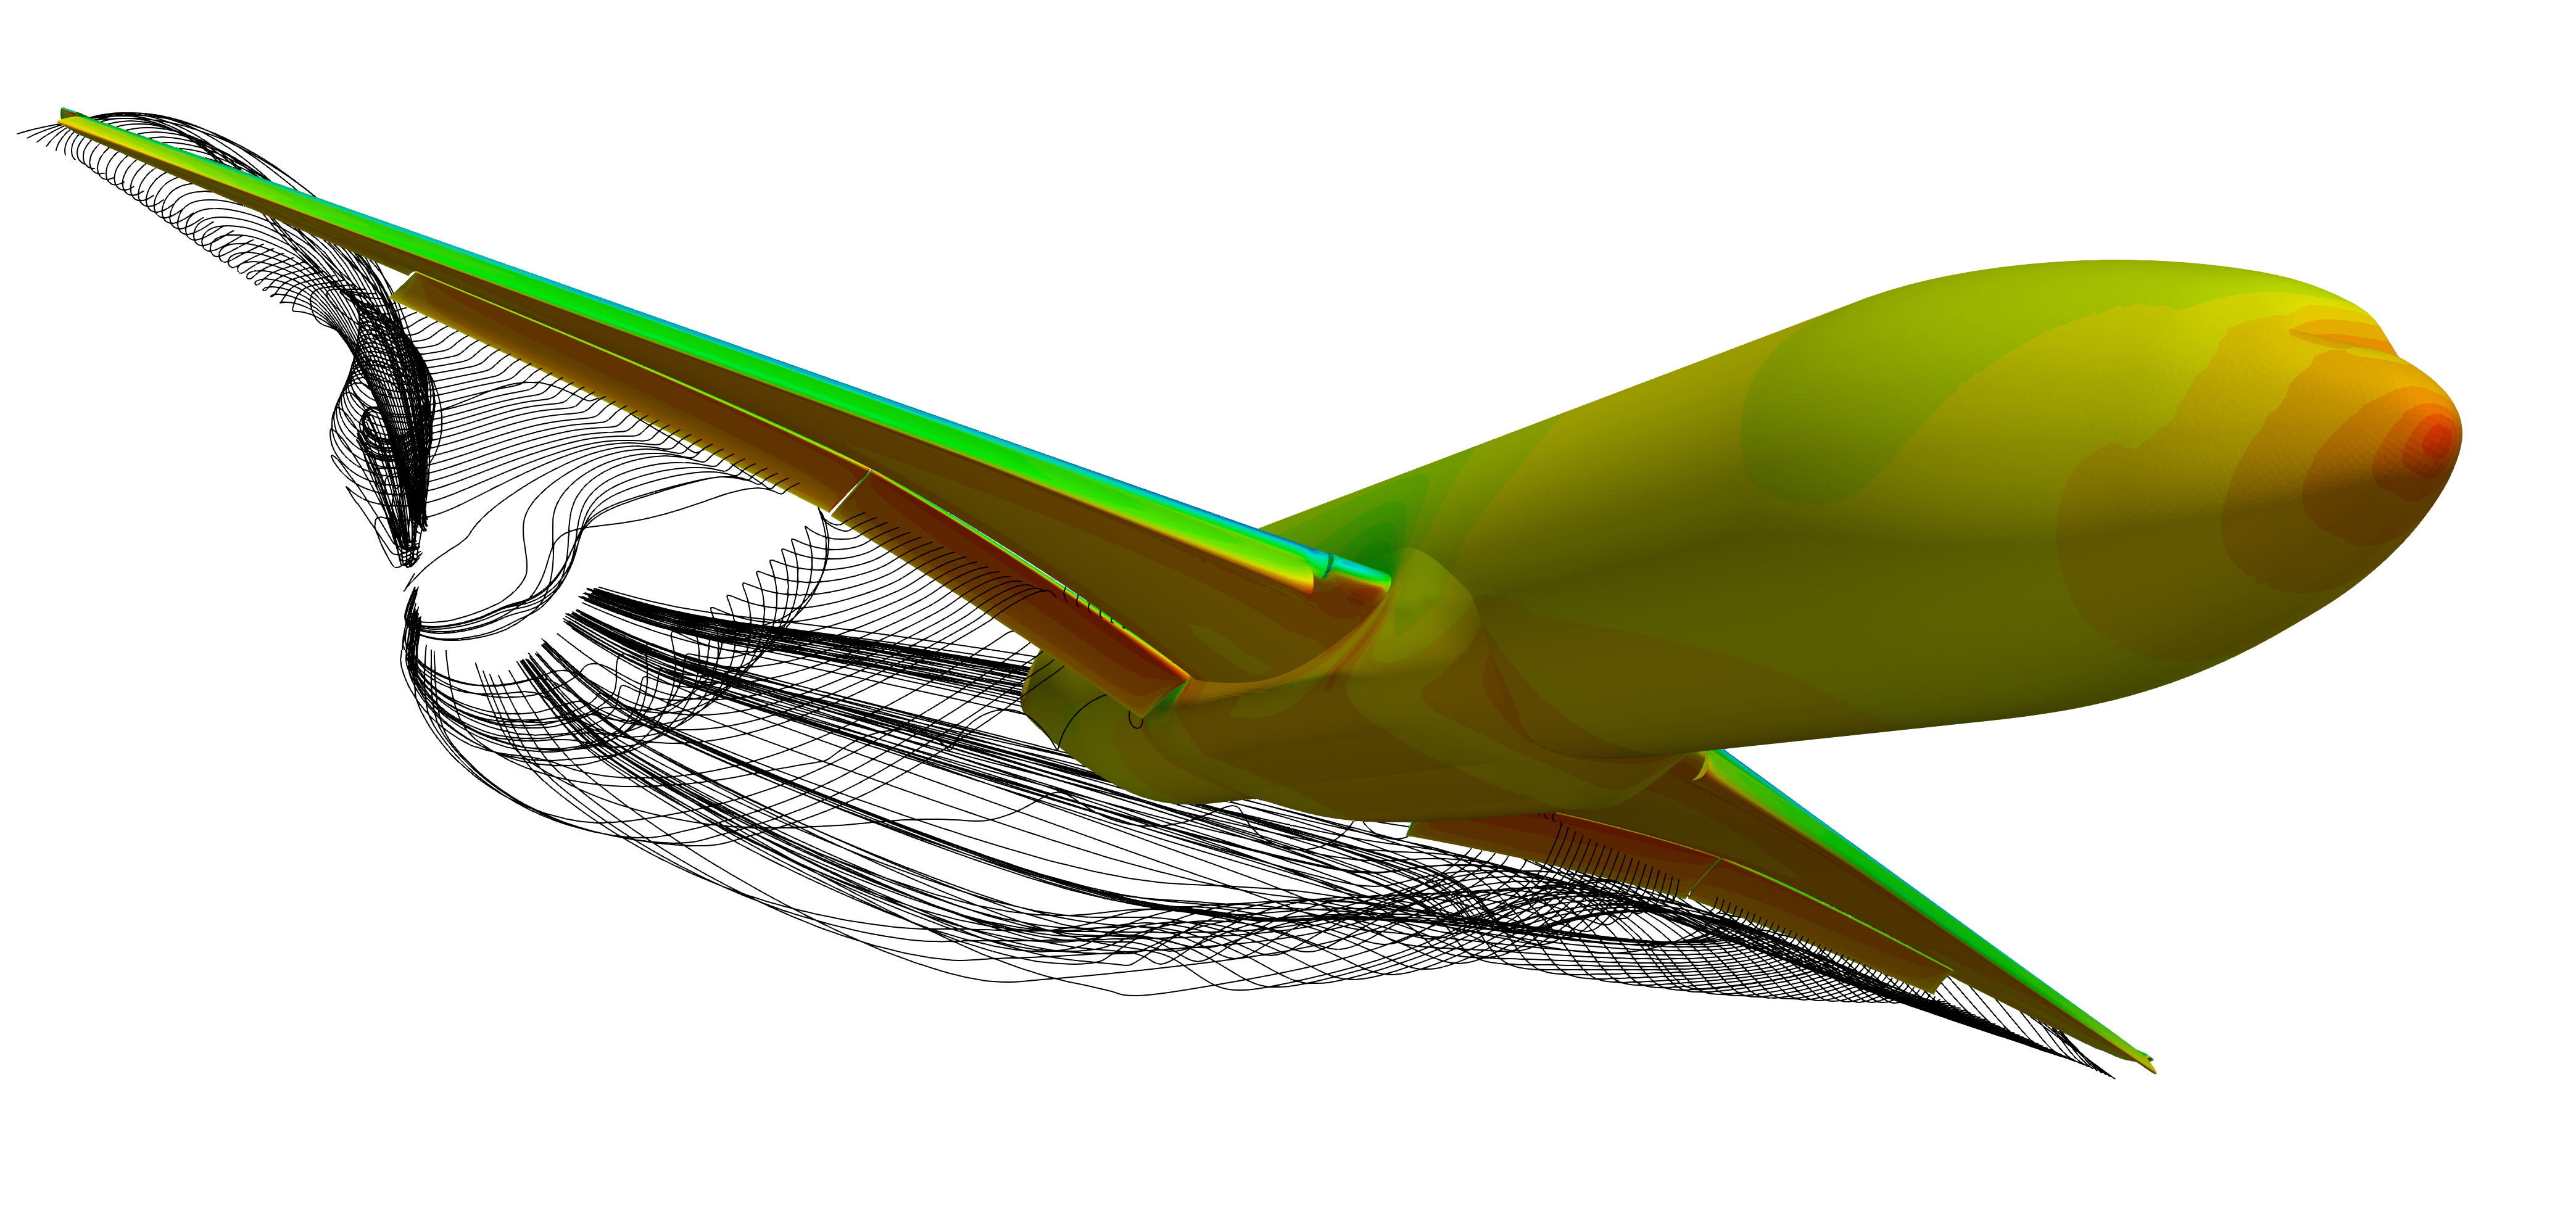
\includegraphics[width=1.15\textwidth]{Figures/hl_crm_01.png}}
\end{figure}

\newpage
\pagenumbering{roman}
\begin{figure}
    \centering
    
\includegraphics[width=6cm]{Figures/logoSU2_v3_3.png}
    %\caption{SU2 official logo}
\end{figure}
    
\tableofcontents 

\newpage

\pagenumbering{arabic}
\pagestyle{fancy}

\section{Configuration File}

The configuration file is a text file that contains a user’s options for a particular problem to be solved with the SU2 suite. It is specified as an input upon execution of SU2 components. This section briefly describes the file format and other conventions.

The SU2 configuration file name typically carries a name of the form filename.cfg. The file extension .cfg is optional (this is our own convention), and the prefix can be any valid string with no spaces; e.g. config.cfg, su2-config.cfg, and flow\_config.cfg are all suitable file names.

The configuration file consists of only three elements:
\begin{enumerate}
    \item \textbf{Options}. An option in the file has the following syntax: option-name = value, where option-name is the name of the option and value is the desired option value. The value element may be a scalar data type, a list of data types, or a more complicated structure. The “=” sign must come immediately after the option-name element and is not optional. Lists of data types may be formatted for appearance using commas, ( )-braces, \{ \}-braces, and [ ]-braces, though this is not required. Semicolons are semantically relevant for several option types and may not be used as convenience delimiters. SU2 will exit with an error if there are options in the config file which do not exist or if there are options with improper formatting. Some example option formats are given below. 
    \begin{enumerate}
        \item \texttt{FREESTREAM\_VELOCITY = ( 5.0, 0.00, 0.00 ) \% braces and commas \\can be used for list options}
        \item \texttt{REF\_ORIGIN\_MOMENT = 0.25 0.0 0.0 \% however, braces and commas \\are verb optional for lists}
        \item \texttt{KIND\_TURB\_MODEL = NONE \% space between elements is \\not significant}

    \end{enumerate}
    \item \textbf{Comments}. On a given line in the file, any text appearing after a \% is considered a comment and is ignored by SU2. Additional \% signs after the first on a given line are not significant.
    \item \textbf{White space}. Empty lines are ignored. On text lines that define options, white space (tabs, spaces) can be used to format the appearance of the file
\end{enumerate}

SU2 includes strict error checking of the config file upon execution of one of the C++ modules. For example, the code will throw errors if unknown options are specified, options appear more than once, extra text appears outside of comments, etc.


\newpage
\section{Mesh File}
SU2 mainly uses a native mesh file format as input into the various suite components. Support for the CGNS data format has also been included as an input mesh format. CGNS support can be useful when it is necessary to create complex geometries in a third-party mesh generation package that can export CGNS files. A converter from CGNS to the native format is also built into SU2. Details on how to create and use these mesh formats is given below.

\subsection{SU2 Native Format (.su2)}
In keeping with the open-source nature of the project, SU2 features its own native mesh format. The format is meant to be simple and readable. A description of the mesh and some examples are below.

\subsubsection{Description}

The SU2 mesh format carries an extension of .su2, and the files are in a readable ASCII format. As an unstructured code, SU2 requires information about both the node locations as well as their connectivity. The connectivity description provides information about the types of elements (triangle, rectangle, tetrahedron, hexahedron, etc.) that make up the volumes in the mesh and also which nodes make up each of those elements. Lastly, the boundaries of the mesh, or markers, are given names, or tags, and their connectivity is specified in a similar manner as the interior nodes.

\subsubsection{Specification}

Consider the following simple, 2D mesh for a square domain consisting of 8 triangular elements. It will be used to explain the .su2 mesh format.

\begin{center}
    \includegraphics[width=9cm]{fig1.png}
\end{center}

\textbf{Square Mesh Example: Note that the figure uses Tecplot node and element number (1-based). The node and element numbering for SU2 start at 0.}

The first line of the .su2 mesh declares the dimensionality of the problem. SU2 can handle 2D or 3D geometries. As a note, for 2D simulations, it is recommended that a truly 2D mesh is used (no z-coordinates) rather than a quasi-2D mesh (one or more cells deep in the third dimension with symmetry boundary conditions). For the 2D square mesh, the dimension is defined as follows:

\begin{lstlisting}
NDIME= 2
\end{lstlisting}


SU2 searches specifically for the keyword \verb|NDIME=| in order to set the dimension, and the dimension value will be stored for use throughout the code. This value would be 3 for a 3D mesh. Note that while “\%” is used here to denote comments, SU2 does not officially recognize it as such. Extra text added to the mesh file between sections (such as lines following a “\%”) will simply be ignored.

To specify the point list, SU2 first searches for the string \verb|NPOIN=| and stores the total number of nodes in the mesh. This value is given first, as it is used to set up a loop over all of the grid points that must immediately follow this line. Then, the coordinates for each of the nodes are given. This is specified in the .su2 format as:

\begin{lstlisting}
NPOIN= 9
0.00000000000000 0.00000000000000
0.50000000000000 0.00000000000000
1.00000000000000 0.00000000000000
0.00000000000000 0.50000000000000
0.50000000000000 0.50000000000000
1.00000000000000 0.50000000000000
0.00000000000000 1.00000000000000
0.50000000000000 1.00000000000000
1.00000000000000 1.00000000000000
\end{lstlisting}


In this case, there are 9 nodes in the 3x3 square above. Immediately after the node number specification comes the list of node coordinates in cartesian space. Each line gives the coordinates for a single grid vertex. The grid points are assigned a global element index of 0 through 8 in the order they appear in the file. This global element index is implied by the ordering and does not need to be explicitly specified by the file, although some legacy meshes may still contain an explicit index at the end of the line that can be ignored.

For a 2D mesh, only x and y coordinates are required, but a 3D mesh would give x, y, and z coordinates. The global index values for the nodes and elements stored within SU2 are zero-based, as opposed to starting from 1 as Tecplot does. The global index numbering of the nodes is implicit in the order they are given in the file. For example, the point (0.0,0.0), the first in the list given in the mesh file, will carry global index 0, the point (0.5,0.0) carries global index 1, and so on. Therefore, the location of each node in the list above can be confirmed in space by adding 1 to the implied global index from the ordering and comparing with the figure above.

The next part of the file describes the interior element connectivity, which begins with the \verb|NELEM=| keyword:
\begin{lstlisting}
NELEM= 8
5 0 1 3
5 1 4 3
5 1 2 4
5 2 5 4
5 3 4 6
5 4 7 6
5 4 5 7
5 5 8 7
\end{lstlisting}


SU2 is based on unstructured mesh technology, and thus supports several element types for both 2D and 3D elements. Unlike for structured meshes where a logical, ordered indexing can be assumed for neighboring nodes and their corresponding cells (quadrilaterals in 2D and hexahedral elements in 3D), for an unstructured mesh, a list of nodes that make up each element, or the connectivity as it is often called, must be provided. First, SU2 will search for the string \verb|NELEM=| and then store the number of interior elements. This value is given first, as it is used to set up a loop over all of the elements which must immediately follow this line. For the square mesh above, this corresponds to the 8 triangular interior elements that are assigned a global element index of 0 through 7 in the order they appear in the file. This global element index is implied by the ordering and does not need to be explicitly specified by the file, although some legacy meshes may still contain an explicit index at the end of the line that can be ignored.

Each following line describes the connectivity of a single element. The first integer on each line is a unique identifier for the type of element that is described. SU2 supports line, triangle, quadrilateral, tetrahedral, pyramid, prism, and hexahedral elements. The identifiers follow the VTK format:


\begin{center}
    \begin{tabular}{| m{12em} | m{17em} |}
    \textbf{Element Type} & \textbf{Identifier}  \\ [0.5ex]
    \hline\hline 
    Line & 3 \\ [1ex]
    \hline
    Triangle & 5 \\ [1ex]
    \hline
    Quadrilateral & 9\\ [1ex]
    \hline
    Tetrahedral & 10 \\ [1ex]
    \hline
    Hexahedral & 12 \\ [1ex]
    \hline
    Prism & 13 \\ [1ex]
    \hline
    Pyramid & 14 \\ [1ex]
    \hline

    \end{tabular}
\end{center}


In our square mesh, all elements are triangles, and thus the identifier (first integer) on all lines is 5. Following the identifier is a list of the node indices that make up the element. Each triangular element will have 3 nodes specified, a rectangular element would have 4 nodes specified, a tetrahedral element would have 4 nodes specified, and so on. Note again that the global index values for the nodes and elements stored within SU2 are zero-based, as opposed to starting from 1 as Tecplot does, which was used to create the mesh image. For example, take the triangular element described in the first line, which would be indexed as 0 in SU2 (1 in Tecplot). The SU2 nodes are given as (0,1,3) which would correspond to (1,2,4) in Tecplot. Looking at the figure of the mesh above, we see that this is the lower left triangular element. The ordering of the nodes given in the connectivity list for a specific element is important, and the user is referred to the VTK format guide for the correct ordering for each supported element type (page 9).

The final component of the mesh is a description of all boundaries (which we call markers), including a name (what we call a tag). For each boundary, the connectivity information is specified using the same node global index values given above. For a 2D mesh, only line elements are supported along the boundaries. For a 3D mesh, triangular and quadrilateral elements are the possible options for boundary elements. This section of the .su2 mesh file appears as:

\begin{lstlisting}
NMARK= 4
MARKER_TAG= lower
MARKER_ELEMS= 2
3 0 1
3 1 2
MARKER_TAG= right
MARKER_ELEMS= 2
3 2 5
3 5 8
MARKER_TAG= upper
MARKER_ELEMS= 2
3 8 7
3 7 6
MARKER_TAG= left
MARKER_ELEMS= 2
3 6 3
3 3 0
\end{lstlisting}


First, the number of boundaries, or markers, is specified using the “NMARK=” string. Then for each marker, a name, or tag, is specified using “MARKER\_TAG=.” This tag can be any string name, and the tag name is used in the configuration file for the solver when specifying boundary conditions. Here, the tags “lower,” “right,” “upper,” and “left” would be used. The number of elements on each marker, using “MARKER\_ELEMS=,” must then be specified before listing the connectivity information as is done for the interior mesh elements at the start of the file. Again, the unique VTK identifier is given at the start of each line followed by the node list for that element. For our example, only line elements (identifier 3) exist along the markers, and on each boundary of the square there are 2 edges of a triangle that make up the marker. These elements can again be verified with the mesh figure above.


\subsubsection{Examples}

Attached here is the simple square mesh from above in .su2 format, along with codes for creating this file in the Python, C++, and Fortran 90 programming languages. These scripts are meant to be examples of how to write .su2 meshes in a few common languages which can be easily modified for creating new meshes:

\begin{itemize}
    \item Square mesh: \href{run:./square.su2}{square.su2}
    \item Python square mesh generator: \href{run:./square.py}{square.py}
    \item C++ square mesh generator: \href{run:./square.cpp}{square.cpp}
    \item Fortran 90 square mesh generator: \href{run:./square.f90}{square.f90}
    
\end{itemize}
   

\subsection{CGNS Format}

To make creating your own meshes easier and more accessible, support for the open CGNS data standard has been included within SU2. The main advantage gained is that complex meshes created in a third-party software package (one that supports unstructured, single-zone CGNS file export in ADF format) can be used directly within SU2 without the need for conversion to the native format. Moreover, as CGNS is a binary format, the size of the mesh files can be significantly reduced.

\subsubsection{Compiling with CGNS Support}

Starting with SU2 v4.3, the source code of the CGNS library is shipped with SU2 in the externals/ directory, and it is automatically built and linked for you when compiling SU2 (ADF support only).


\subsubsection{Using and Converting CGNS Meshes}

In order to use a CGNS mesh (assuming the CGNS library has been installed and SU2 successfully compiled), the user simply needs to specify the input mesh format to be “CGNS” in the configuration file for their simulation. The configuration file option is “MESH\_FORMAT=” and appears as:

\begin{lstlisting}
MESH_FORMAT= CGNS
\end{lstlisting}


It is important to note that SU2 will not use any specific boundary conditions that are embedded within the CGNS mesh. However, it will use the names given to each boundary as the marker tags. These marker tags are used to set the boundary conditions in the configuration file. Therefore, it is recommended that the user give names to each boundary in their mesh generation package before exporting to CGNS. If you do not know the number of markers or their tags within a CGNS file, you can simply attempt a simulation in SU2\_CFD (leaving out the boundary information in the configuration file at first), and during the preprocessing stage, SU2 will read and print the names of all boundary markers to the console along with other grid information before throwing an error due to incomplete boundary definitions. The user can then incorporate these marker tags into the configuration file with the appropriate boundary conditions.

If needed, a converter from CGNS to the SU2 format has been built into SU2 (See the inviscid wedge tutorial).

\subsection{Third-Party Mesh Software}


We are continuously working to integrate SU2 with industry-standard tools. The latest releases of the Pointwise meshing software can both export and import meshes in the native ASCII SU2 format. In addition, a number of other packages support direct output to the SU2 format, such as GMSH and CENTAUR. CGNS files created by a number of other meshing packages have been successfully tested and used, such as those from ICEM CFD, for instance.

\newpage

\section{Restart File}
The SU2 binary restart format has the extension \verb|.dat|, but it is also possible to write out restart files in a simple ASCII file format with extension \verb|.csv|. Have a look at the Output section to learn how to change output file formats.

The restart files are used to restart the code from a previous solution and also to run the adjoint simulations, which require a flow solution as input. In order to run an adjoint simulation, the user must first change the name of the \verb|restart_flow.dat| file (or \verb|restart_flow.csv| if ASCII format) to \texttt{solution\_flow.dat} (or \verb|solution_flow.csv|) in the execution directory (these default file names can be adjusted in the config file). It is important to note that the adjoint solver will create a different adjoint restart file for each objective function, e.g. \verb|restart_adj_cd.dat|.

To restart a simulation the \verb|RESTART_SOL| flag should be set to \verb|YES| in the configuration file. If performing an unsteady restart the \verb|RESTART_ITER| needs to be set to the iteration number which you want to restart from. For instance if we want to restart at iteration 100 and run the unsteady solver with 2nd-order dual time stepping method, we will need to specify \verb|RESTART_ITER = 100| and have the restart files \verb|solution_flow_00098.dat| and \verb|solution_flow_00099.dat|.


\newpage
\section{Solver Setup}
\begin{adjustbox}{width=\textwidth}
\begin{tabular}{ m{12em} | m{17em}| m{13em} }
% \begin{adjustbox}{tabular= m{12em} | m{19em}| m{10em} ,center}
     \textbf{Option Value} & \textbf{Problem} & \textbf{Type} \\ [0.5ex]
    \hline\hline 
    EULER & \textbf{Euler's equation} & Finite-Volume method \\ [1ex]
    
    NAVIER\_{STOKES} & \textbf{Navier-Stokes' equation} & Finite-Volume method \\ [1ex]
    
    RANS & \textbf{Reynolds-averaged Navier-Stokes' equation} & Finite-Volume method \\ [1ex]
    
    INC\_{}EULER & \textbf{Incompressible Euler's equation} & Finite-Volume method \\ [1ex]
    
    INC\_{}NAVIER\_{}STOKES & \textbf{Incompressible Navier-Stokes' equation} & Finite-Volume method \\ [1ex]
    
    INC\_{}RANS & \multirow{2}{20em}{\textbf{Incompressible Reynolds-averaged Navier-Stokes' equation}} & Finite-Volume method \\ [1ex]
    
    & & \\ [1ex]
    
    HEAT\_{}EQUATION\_FM & \textbf{Heat equation} & Finite-Volume method \\ [1ex]
    
    ELASTICITY & \textbf{Equations of elasticity} & Finite-Volume method \\ [1ex]
     
    FEM\_EULER & \textbf{Euler's equation} & Discontinuos Galerkin FEM \\ [1ex]
    
    FEM\_NAVIER\_STOKES & \textbf{Navier-Stokes' equation} & Discontinuos Galerkin FEM \\ [1ex]
    
    MULTIPHYSICS & Multi-zone problem with different solvers in each zone & - \\
    \hline
    \end{tabular}
\end{adjustbox}

\iffalse
\begin{center}
    \begin{tabular}{ m{12em} | m{17em}| m{13em} }
    \textbf{Option Value} & \textbf{Problem} & \textbf{Type} \\ [0.5ex]
    \hline\hline 
    EULER & \textbf{Euler's equation} & Finite-Volume method \\ [1ex]
    
    NAVIER\_{STOKES} & \textbf{Navier-Stokes' equation} & Finite-Volume method \\ [1ex]
    
    RANS & \textbf{Reynolds-averaged Navier-Stokes' equation} & Finite-Volume method \\ [1ex]
    
    INC\_{}EULER & \textbf{Incompressible Euler's equation} & Finite-Volume method \\ [1ex]
    
    INC\_{}NAVIER\_{}STOKES & \textbf{Incompressible Navier-Stokes' equation} & Finite-Volume method \\ [1ex]
    
    INC\_{}RANS & \multirow{2}{20em}{\textbf{Incompressible Reynolds-averaged Navier-Stokes' equation}} & Finite-Volume method \\ [1ex]
    
    & & \\ [1ex]
    
    HEAT\_{}EQUATION\_FM & \textbf{Heat equation} & Finite-Volume method \\ [1ex]
    
    ELASTICITY & \textbf{Equations of elasticity} & Finite-Volume method \\ [1ex]
     
    FEM\_EULER & \textbf{Euler's equation} & Discontinuos Galerkin FEM \\ [1ex]
    
    FEM\_NAVIER\_STOKES & \textbf{Navier-Stokes' equation} & Discontinuos Galerkin FEM \\ [1ex]
    
    MULTIPHYSICS & Multi-zone problem with different solvers in each zone & - \\ [1ex]
    \end{tabular}
\end{center}

\fi 

\vspace{2mm}
Every solver has its specific options and we refer to the tutorial cases for more information. However, the basic controls detailed in the remainder of this page are the same for all problems.

\subsection{Restarting the simulation}
A simulation can be restarted from a previous computation by setting \texttt{RESTART\_SOL \\= YES}. If it is a time-dependent problem, additionally \verb|RESTART_ITER| must be set to the time iteration index you want to restart from: 

\begin{lstlisting}
% --------------------- Solver definition ---------------------- %
%
% Type of solver 
SOLVER= EULER
%
% Restart solution (NO, YES)
RESTART_SOL= NO
%
% Iteration number to begin unsteady restarts (used if RESTART_SOL= YES)
RESTART_ITER= 0
%

\end{lstlisting}

\newpage
\subsection{Controlling the simulation}
A simulation is controlled by setting the number of iterations the solver should run (or by setting a convergence critera). The picture below depicts the two types of iterations we consider.

\begin{center}
    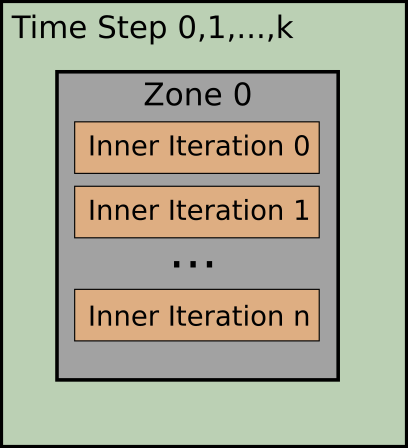
\includegraphics[width=6cm]{Figures/unst_singlezone.png}
\end{center}

SU2 makes use of an outer time loop to march through the physical time, and of an inner loop which is usually a pseudo-time iteration or a (quasi-)Newton scheme. The actual method used depends again on the specific type of solver.

\subsection{Time-dependent Simulation}
To enable a time-dependent simulation set the option \verb|TIME_DOMAIN| to \verb|YES| (default is \verb|NO|). There are different methods available for certain solvers which can be set using the \verb|TIME_MARCHING| option. For example for any of the FVM-type solvers a first or second-order dual-time stepping (\texttt{DUAL\_TIME\_STEPPING-1ST\_ORDER} or \texttt{DUAL\_TIME\_STEPPING\-2ND\_ORDER}) method or a conventional time-stepping method (\verb|TIME_STEPPING|) can be used.

\begin{lstlisting}
% ---------------- Time-dependent Simulation -------------------- %
%
TIME_DOMAIN= YES
%
% Time Step for dual time stepping simulations (s)
TIME_STEP= 1.0
%
% Total Physical Time for dual time stepping simulations (s)
MAX_TIME= 50.0
%
% Number of internal iterations 
INNER_ITER= 200
%
% Number of time steps
TIME_ITER= 200
%
\end{lstlisting}


The solver will stop either when it reaches the maximum time (\verb|MAX_TIME|) or the maximum number of time steps (\verb|TIME_ITER|), whichever event occurs first. Depending on the \verb|TIME_MARCHING| option, the solver might use an inner iteration loop to converge each physical time step. The number of iterations within each time step is controlled using the \verb|INNER_ITER| option.


\subsection{Steady-state Simulation}
A steady-state simulation is defined by using \verb|TIME_DOMAIN = NO|, which is the default value if the option is not present. In this case the number of iterations is controlled by the option \verb|ITER|.

Note: To make it easier to switch between steady-state, time-dependent and multizone simulations, the option \verb|INNER_ITER |can also be used to specify the number of iterations. If both options are present, \verb|INNER_ITER| has precedence

\subsection{Setting convergence criteria}
Despite setting the maximum number of iterations, it is possible to use a convergence criterion so that the solver will stop when it reaches a certain value of a residual or if variations of a coefficient are below a certain threshold. To enable a convergence criterion use the option \verb|CONV_FIELD| to set an output field that should be monitored. The list of possible fields depends on the solver. Take a look at Custom Output to learn more about output fields. Depending on the type of field (residual or coefficient) there are two types of methods:

\subsubsection{Steady-state Residual}

If the field set with \verb|CONV_FIELD| is a residual, the solver will stop if it is smaller than the value set with \verb|CONV_RESIDUAL_MINVAL| option. Example:


\begin{lstlisting}
% ------------ Residual-based Convergence Criteria -------------- %
%
CONV_FIELD= RMS_DENSITY
%
%
% Min value of the residual (log10 of the residual)
CONV_RESIDUAL_MINVAL= -8
%
\end{lstlisting}

\subsubsection{Steady-state Coefficient}

If the field set with \verb|CONV_FIELD| is a coefficient, a Cauchy series approach is applied. A Cauchy element is defined as the relative difference of the coefficient between two consecutive iterations. The solver will stop if the average over a certain number of elements (set with \verb|CONV_CAUCHY_ELEMS|) is smaller than the value set with \verb|CONV_CAUCHY_EPS|. The current value of the Cauchy coefficient can be written to screen or history by adding the \verb|CAUCHY| field to the \verb|SCREEN_OUTPUT| or \verb|HISTORY_OUTPUT| option (see Custom Output). Example:


\begin{lstlisting}
% ---------- Coefficient-based Convergence Criteria ------------- %
%
CONV_FIELD= DRAG
%
%
% Number of elements to apply the criteria
CONV_CAUCHY_ELEMS= 100
%
% Epsilon to control the series convergence
CONV_CAUCHY_EPS= 1E-10
%

\end{lstlisting}
For both methods the option \verb|CONV_STARTITER| defines when the solver should start monitoring the criterion


\subsubsection{Time-dependent Coefficient}

In a time-dependend simulation we have two iterators, \verb|INNER_ITER| and \verb|TIME_ITER|. The convergence criterion for the \verb|INNER_ITER| loop is the same as in the steady-state case. For the \verb|TIME_ITER|, there are convergence options implemented for the case of a periodic flow. The convergence criterion uses the so-called windowing approach, (see Custom Output). The convergence options are applicable only for coefficients. To enable time convergence, set \verb|WINDOW_CAUCHY_CRIT=YES| (default is \verb|NO|). The option \verb|CONV_WINDOW_FIELD| determines the output-fields to be monitored. Typically, one is interested in monitoring time-averaged coefficients, e.g \verb|TAVG_DRAG|. Analogously to the steady state case, the solver will stop, if the average over a certain number of elements (set with \verb|CONV_WINDOW_CAUCHY_ELEMS|) is smaller than the value set with \verb|CONV_WINDOW_CAUCHY_EPS|. The current value of the Cauchy coefficient can be written to screen or history using the flag \verb|CAUCHY |(see Custom Output). The option \verb|CONV_WINDOW_STARTITER| determines the numer of iterations, the solver should wait to start moniotring, after \verb|WINDOW_START_ITER| has passed.

\texttt{WINDOW\_START\_ITER} determines the iteration, when the (time dependent) outputs are averaged, (see Custom Output). The window-weight-function used is determined by the option \verb|WINDOW_FUNCTION|


\begin{lstlisting}

% ---- Coefficient-based Windowed Time Convergence Criteria ---- %
%
% Activate the windowed cauchy criterion
WINDOW_CAUCHY_CRIT = YES
%
% Specify convergence field(s)
CONV_WINDOW_FIELD= (TAVG_DRAG, TAVG_LIFT)
%
% Number of elements to apply the criteria
CONV_WINDOW_CAUCHY_ELEMS= 100
%
% Epsilon to control the series convergence
CONV_WINDOW_CAUCHY_EPS= 1E-3
%
% Number of iterations to wait after the iteration specified in  WINDOW_START_ITER.
CONV_WINDOW_STARTITER = 10
%
% Iteration to start the windowed time average
WINDOW_START_ITER = 500
%
% Window-function to weight the time average. Options (SQUARE, HANN, HANN_SQUARE, BUMP), SQUARE is default.
WINDOW_FUNCTION = HANN_SQUARE
%

\end{lstlisting}

Note: The options \verb|CONV_FIELD| and \verb|CONV_WINDOW_FIELD| also accept a list of fields, e.g. \verb|(DRAG, LIFT,...)|, to monitor. The solver will stop if all fields reach their respective stopping criterion (i.e. the minimum value for residuals or the cauchy series threshold for coefficients as mentioned above).

\newpage
\section{Physical Definition}
The physical definition of a case includes the definition of the free-stream, the reference values and the non-dimensionalization. SU2 offers different ways of setting and computing this definition. This document gives a short overview on the config options and their physical relation.

\subsection{Reference Values}
The following table depicts the reference values used by most of the solvers in SU2. The highlighted variables vary depending on the actual solver and the user input.

\begin{center}
\begin{tabular}{{ m{13em}  m{5em} m{12em} }}

\textbf{Variable} & \textbf{Unit} & \textbf{Reference} \\[1ex]
 \hline\hline
 Length & \(m\) & \(l_{ref} = 1\) \\ [1ex]
 \hline
 \textbf{Density} & \(\frac{kg}{m^3}\) & \(\rho_{ref}\) (based on user input) \\ [1ex]
 \hline 
 \textbf{Velocity} & \(\frac{m}{s}\) & \(v_{ref}\) (based on user input)\\ [1ex]
 \hline 
 \textbf{Temperature} & \(K\) & \(T_{ref}\) (based on user input) \\ [1ex]
 \hline 
 \textbf{Pressure} & \(Pa\) & \(p_{ref}\) (based on user input) \\ [1ex]
 \hline
  Viscosity & \(\frac{kg}{ms}\) & \(\mu_{ref}\) (based on user input) \\[1ex]
  \hline
  Time & \(s\) & \(t_{ref} = \frac{l_{ref}}{v_{ref}}\) \\ [1ex]
 \hline
 Heatflux & \(\frac{W}{m^2}\) & \(Q_{ref} = \rho_{ref}v_{ref}^3\) \\ [1ex]
 \hline
 Gas constant & \(\frac{m^2}{s^2K}\) & \(R_{ref} = \frac{v_{ref}^2}{T_{ref}}\) \\ [1ex]
 \hline
 Conductivity & \(\frac{W}{mK}\) & \(k_{ref} = \mu_{ref}R_{ref}\) \\ [1ex]
 \hline
 Force & \(N\) & \(F_{ref} = \rho_{ref}v_{ref}^2l_{ref}^2\) \\ [1ex]
 \hline
 \hline
\end{tabular}
\end{center}


\subsection{Free-Stream Definition (Compressible)}
	The physical definition for the compressible solvers in SU2 based around the definition of the free-stream. The free-stream values are not only used as boundary conditions for the \verb|MARKER_FAR| option, but also for initialization and non-dimensionalization. That means even if you don’t have any farfield BCs in your problem, it might be important to prescribe physically meaningful values for the options.

\subsubsection{Thermodynamic State}

The thermodynamic state of the free-stream is defined by the pressure \(p_\infty\), the density \(\rho_\infty\) and the temperature \(T_\infty\). Since these quantities are not independent, only two of these values have to be described and the third one can be computed by an equation of state, depending on the fluid model used. There are two possible ways implemented that can be set using \verb|FREESTREAM_OPTION|:

\begin{itemize}
    \item \verb|TEMPERATURE_FS| (default): Density \(\rho_\infty\) is computed using the specified pressure \(p_\infty\) \\(\verb|FREESTREAM_PRESSURE|) and temperature \(T_\infty\) (\verb|FREESTREAM_TEMPERATURE|).
    \item \verb|DENSITY_FS|: Temperature \(T_\infty\) is computed using the specified pressure \(p_\infty\) \\ (\verb|FREESTREAM_PRESSURE|) and density \(\rho_\infty\) (\verb|FREESTREAM_DENSITY|).
\end{itemize}


\subsubsection{Mach Number and Velocity}

The free-stream velocity \(v_\infty\) is always computed from the specified Mach number \(Ma_\infty\)  (\verb|MACH_NUMBER|) and the computed thermodynamic state. The flow direction is based on the angle of attack (\verb|AOA|) and the side-slip angle (\verb|SIDESLIP_ANGLE|, for 3D).


\subsubsection{Reynolds Number and Viscosity}

If it is a viscous computation, by default the pressure \(p_\infty\) will be recomputed from a density \(\rho_\infty\) that is found from the specified Reynolds number \(Re\) (\verb|REYNOLDS_NUMBER|). Note that for an ideal gas this does not change the Mach number \(Ma_\infty\) as it is only a function of the temperature \(t_\infty\). If you still want to use the thermodynamic state for the free-stream definition, set the option \verb|INIT_OPTION| to \verb|TD_CONDITIONS| (default: \verb|REYNOLDS|). In both cases, the viscosity is computed from the dimensional version of Sutherland’s law or the constant viscosity (\verb|FREESTREAM_VISCOSITY|), depending on the \verb|VISCOSITY_MODEL| option.


\subsubsection{Non-Dimensionalization}

For all schemes, as reference values for the density and temperature the free-stream values are used, i.e. \(\rho_{ref} = \rho_\infty, T_{ref} = T_\infty\). The reference velocity is based on the speed of sound defined by the reference state: \(v_{ref} = \sqrt{\frac{p_{ref}}{\rho_{ref}}}\). The dimensionalization scheme can be set using the option \verb|REF_DIMENSIONALIZATION| and defines how the reference pressure \(p_{ref}\) is computed:

\begin{itemize}
    \item \verb|DIMENSIONAL|: All reference values are set to \verb|1.0|, i.e. the computation is dimensional.
    \item \verb|FREESTREAM_PRESS_EQ_ONE|: Reference pressure equals free-stream pressure, \(p_{ref} = p_\infty\).
    \item \texttt{FREESTREAM\_VEL\_EQ\_MACH}: Reference pressure is chosen such that the non dimensional free-stream velocity equals the Mach number: \(p_{ref} = \gamma p_\infty\).
    \item \verb|FREESTREAM_VEL_EQ_ONE|: Reference pressure is chosen such that the non dimensional free-stream velocity equals \verb|1.0|: \(p_{ref} = Ma_\infty^2\gamma p_\infty\).
\end{itemize}


\subsection{Flow Condition (Incompressible)}

The physical definition of the incompressible solvers is accomplished by setting an appropriate flow condition for initialization and non-dimensionalization. SU2 solves the incompressible Navier-Stokes equations in a general form allowing for variable density due to heat transfer through the low-Mach approximation (or incompressible ideal gas formulation).
\subsubsection{Thermodynamic and Gauge Pressure}

In the incompressible problem the thermodynamic pressure is decoupled from the governing equations and density is therefore only a function of temperature variations. The absolute value of the pressure is not important and any reference to the pressure \(p\) is considered as the gauge value, i.e. it is zero-referenced against ambient air pressure, so it is equal to absolute pressure minus (an arbitrary) atmospheric pressure.

\subsubsection{Initial State and Non-Dimensionalization}

The initial state, i.e. the initial values of density \(\rho_0\), velocity vector \(\overrightarrow{v_0}\) and temperature \(t_0\) are set with \verb|INC_DENSITY_INIT|, \verb|INC_VELOCITY_INIT| and \\ \verb|INC_TEMPERATURE_INIT|, respectively. The initial pressure \(p_0\) is always set to \verb|0.0|.

The reference values \(v_{ref}, T_{ref}, v_{ref}\) equal the initial state values by default (or if \texttt{INC\_NONDIM = INITIAL\_VALUES}). If \verb|INC_NONDIM| is set to \verb|REFERENCE_VALUES| you can define different values for them using the options \verb|INC_DENSITY_REF|, \verb|INC_VELOCITY_REF| and \verb|INC_TEMPERATURE_REF|. The reference pressure is always computed by \(p_{ref} = \rho_{ref}v_{ref}^2\).\\
\vspace{.1em}

\textbf{NOTE}: The initial state is also used as boundary conditions for \verb|MARKER_FAR|.

\newpage
\section{Markers and Boundary Conditions}

The term Marker refers to a named entity in your mesh file. Boundary conditions are defined by assigning names of the markers to the corresponding option. Below you will find a list of the most common boundary conditions along with a short description.

\subsection{Euler (Slip) Wall}
An Euler wall for inviscid flow is defined with the \verb|MARKER_EULER| option. It can also be used as a slip wall in viscous flow. Only the marker name has to be given for this option.

For all Finite Volume (FVM) solvers, i.e. not the \verb|FEM_*| solvers, its implementation is identical to \verb|MARKER_SYM| solvers and both options can be used interchangeably.

\begin{lstlisting}
MARKER_EULER = (Euler_Wall1, Euler_Wall2, ...)
\end{lstlisting}

\textbf{Note}: Be aware when switching from an Euler solver to a Navier-Stokes one that most solid walls should become \verb|MARKER_HEATFLUX| (and vice versa).

\subsection{Symmetry Wall}
A symmetry wall is defined with using the \verb|MARKER_SYM| option. Only the marker name has to be given for this option.

For all Finite Volume (FVM) solvers, i.e. not the \verb|FEM_*| solvers, its implementation is identical to \verb|MARKER_SYM| solvers and both options can be used interchangeably.

\begin{lstlisting}
MARKER_SYM = (Symmetry_Wall1, Symmetry_Wall2, ...)

\end{lstlisting}


\subsection{Constant Heatflux (no-slip) Wall}
A wall with a prescribed constant heatflux is defined with the \verb|MARKER_HEATFLUX| option. The option format is the marker name followed by the value of the heatflux (in Watts per square meter \verb|[W/m^2],[J/(s*m^2)]|), e.g.

\begin{lstlisting}
MARKER_HEATFLUX = (Wall1, 1e05, Wall2, 0.0)
\end{lstlisting}

\textbf{Note}: Typically Navier-Stokes and RANS simulations are setup with adiabatic walls (heatflux = 0)

\subsection{Heat Transfer or Convection (no-slip) Wall}
A wall with a prescribed locally variable heatflux via a heat transfer coefficient and and a Temperature at infinity (or reservoir Temperature) is defined with the \texttt{MARKER\_HEATTRANSFER} option. The heatflux \verb|q| computes to \verb|q = h(T_inf - T_wall)|, where \verb|T_wall| is the local wall temperature and therefore no user input. The option format is the marker name followed by the value of the heat-transfer coefficient (in Watts per square meter and Kelvin \verb|[W/(m^2*K)],[J/(s*m^2*K)]|) and the value of the Temperature at infinity (in Kelvin \verb|[K]|), e.g.

\begin{lstlisting}
MARKER_HEATTRANSFER = (Wall1, 10.0, 350.0, Wall2, 5.0, 330.0, ...)

\end{lstlisting}


\textbf{Note}: The Heat Transfer Wall degenerates to an adiabatic wall when the heat transfer coefficient is zero. On the other extreme (a very high heat transfer coefficient) the Heat Transfer Wall degenerates to an isothermal wall with Temperature at infinity being the wall temperature.

\subsection{Isothermal (no-slip) Wall}
A wall with a constant temperature is defined with the \verb|MARKER_ISOTHERMAL| option. The option format is the marker name followed by the value of the temperature (in Kelvin \verb|[K]|), e.g.

\begin{lstlisting}
MARKER_ISOTHERMAL = (Wall1, 300.0, Wall2, 250.0)

\end{lstlisting}

\subsection{Farfield Boundary Condition}
A marker can be defined as a Farfield boundary by addings its name to the \verb|MARKER_FAR| option. No other values are necesseary for that option. The actual values which will be prescribed depend on the solver and other user input settings. More details can be found in the Physical Definition section.

\begin{lstlisting}
MARKER_FAR= (farfield)

\end{lstlisting}


\subsection{Inlet Boundary Condition}
Inlet boundary conditions are set using the option \verb|MARKER_INLET|.

\subsubsection{Total Conditions}
To describe the \textbf{Total Conditions} at the inlet, set the option \texttt{INLET\_TYPE = TOTAL\_CONDITIONS} (which is the default). The format for \verb|MARKER_INLET| then is the marker name, followed by the Total Temperature (in Kelvin \verb|[K]|), the total Pressure (in Pascal \verb|[Pa]|) and the flow direction unity vector (in meter per second \verb|[m/s]|). For example:

\begin{lstlisting}

INLET_TYPE= TOTAL_CONDITIONS
MARKER_INLET = (inlet1, 300, 1e6, 1.0, 0.0, 0.0, inlet2, 400, 1e6, 0.0, 1.0, 0.0)

\end{lstlisting}


\subsubsection{Mass Flow Inlet}
To describe the \textbf{Mass Flow} at the inlet, set the option \verb|INLET_TYPE= MASS_FLOW|. The format for \verb|MARKER_INLET| then is the marker name, followed by the Density (in \verb|[kg/m^3]|), the Velocity magnitude (in meter per second \verb|[m/s]|) and the flow direction unity vector (in meter per second \verb|[m/s]|). For example:

\begin{lstlisting}
INLET_TYPE= MASS_FLOW
MARKER_INLET = (inlet1, 1.13 , 20, 1.0, 0.0, 0.0, inlet2, 1.15, 10, 0.0, 1.0, 0.0)

\end{lstlisting}


\textbf{Note}: It is not possible to combine Mass Flow Inlet BCs and Total Condition Inlet BCs yet

\subsubsection{Velocity Inlet}
To describe the \textbf{Velocity} at the inlet, set the option \texttt{INC\_INLET\_TYPE=VELOCITY\_INLET}. The format for \verb|MARKER_INLET| then is the marker name, followed by the Temperature (in Kelvin \verb|[K]|), the Velocity magnitude (in meter per second \verb|[m/s]|) and the flow direction unity vector (in meter per second \verb|[m/s]|).

\begin{lstlisting}
INC_INLET_TYPE= VELOCITY_INLET, VELOCITY_INLET
MARKER_INLET = (inlet1, 300 , 20, 1.0, 0.0, 0.0, inlet2, 200, 10, 0.0, 1.0, 0.0)
\end{lstlisting}


\subsubsection{Pressure Inlet}
To describe the \textbf{Total Pressure} at the inlet, set the option \texttt{INC\_INLET\_TYPE= \\PRESSURE\_INLET}. The format for \verb|MARKER_INLET| then is the marker name, followed by the Temperature (in Kelvin \verb|[K]|), the Total Pressure (in Pascal \verb|[Pa]|) and the flow direction unity vector (in meter per second \verb|[m/s]|).

\begin{lstlisting}
INC_INLET_TYPE= PRESSURE_INLET, PRESSURE_INLET
MARKER_INLET = (inlet1, 300 , 1e6, 1.0, 0.0, 0.0, inlet2, 200, 1e6, 0.0, 1.0, 0.0)
\end{lstlisting}

\textbf{Note 1}: It is possible to combine Velocity Inlet BCs and Pressure Inlet BCs.

\textbf{Note 2}: Updates to the velocity based on the prescribed pressure are damped in order to help with stability/convergence. The damping coefficient can be changed using the \verb|INC_INLET_DAMPING| option (default is \verb|0.1|).


\subsection{Outlet Boundary Condition}
Outlet boundary conditions are set using the \verb|MARKER_OUTLET| option.


\subsubsection{Pressure Outlet (Compressible)}
To describe the static thermodynamic pressure at an outlet, the format for \verb|MARKER_OUTLET| is the marker name, followed by the value of the static pressure (in Pascal \verb|[Pa]|).

\begin{lstlisting}
MARKER_OUTLET = (outlet, 1e5)
\end{lstlisting}


\subsubsection{Pressure Outlet (Incompressible)}
To describe the pressure at an outlet, set the option \texttt{INC\_OUTLET\_TYPE=PRESSURE\_OUTLET}. The format for \verb|MARKER_OUTLET| is the marker name, followed by the value of the gauge pressure (in Pascal \verb|[Pa]|).

\begin{lstlisting}
INC_OUTLET_TYPE= PRESSURE_OUTLET
MARKER_OUTLET = (outlet, 1e1)
\end{lstlisting}

\textbf{Note}: Gauge pressure is zero-referenced against ambient air pressure, so it is equal to absolute pressure minus atmospheric pressure

\subsubsection{Mass Flow Outlet}
To describe the mass flow at an outlet, set the option \texttt{INC\_OUTLET\_TYPE= MASS\_FLOW\_OUTLET}. The format for \verb|MARKER_OUTLET| is the marker name, followed by the value of the target mass flow (in kilogramm per second \verb|[kg/s]|).

\begin{lstlisting}
INC_OUTLET_TYPE= MASS_FLOW_OUTLET
MARKER_OUTLET = (outlet, 1e1)
\end{lstlisting}

\textbf{Note}: Updates to the pressure based on the prescribed mass flow are damped in order to help with stability/convergence. The damping coefficient can be changed using the \verb|INC_OUTLET_DAMPING| option (default is \verb|0.1|).


\subsection{Periodic Boundary Condition}
\subsection{Structural Boundary Conditions}
\subsubsection{Clamped Boundary}
The format for this boundary condition consists of a list of all clamped surfaces (markers). Structural displacements are set to 0 for the nodes on those surfaces.

\begin{lstlisting}
MARKER_CLAMPED = (surface_1,...,surface_N)
\end{lstlisting}

\textbf{Note}: A well posed structural problem requires at least one surface as\\ \verb|MARKER_CLAMPED| or \verb|MARKER_DISPLACEMENT|.

\subsubsection{Displacement Boundary}


The displacements of the nodes on \verb|surface| are enforced, the displacement vector is specified by magnitude and direction (the x/y/z components), internally the solver makes the direction unitary, the multiplier (should usually be set to 1) can be used to increase/decrease the magnitude for example after scaling an existing mesh.

\begin{lstlisting}
MARKER_DISPLACEMENT = (surface, multiplier, magnitude `[m]`, x component, y component, z component)
\end{lstlisting}


\textbf{Note}: Be aware of intersecting surfaces with incompatible displacements, there are shared nodes between adjacent surfaces.

\subsubsection{Load Boundary}

A force-like boundary condition but specified in terms of pressure (units of Pa) which is integrated to obtain nodal forces. The syntax is identical to \verb|MARKER_DISPLACEMENT|.

\begin{lstlisting}
MARKER_LOAD = (surface, multiplier, magnitude `[Pa]`, x component, y component, z component)
\end{lstlisting}


\textbf{Note}: In the context of nonlinear elasticity, this is not a following force.

\subsubsection{Normal Pressure Boundary}

Normal pressure boundary condition (positive means into the surface). This is a following force both magnitude and direction depend of the deformation of the structure.

\begin{lstlisting}
MARKER_PRESSURE = (surface, inward pressure `[Pa]`)
\end{lstlisting}

\newpage
\section{Convective Schemes}
This page lists the convective schemes available in SU2 and their associated options, it is not meant as a detailed theory guide but some application guidance is given nonetheless. The options listed here do not apply to the high order DG solver.

\subsection{Introduction}
Convective schemes are used in the FVM discretization of convective fluxes through the faces of the dual-grid control volumes. They are selected via option \texttt{CONV\_NUM\_METHOD\_FLOW} and fall under the two broad categories of central and upwind. Central schemes tend to be more robust whereas second order upwind schemes can be more accurate (i.e. less dissipative). To achieve second order upwind schemes need to be used with MUSCL reconstruction (\verb|MUSCL_FLOW = YES|), see the “gradients and limiters” page for the MUSCL-related options.

\textbf{Note}: MUSCL options have no effect on central schemes or on coarse multigrid levels in general.


\subsection{Compressible Flow}

\subsubsection{Central Schemes}

\begin{itemize}
    \item \verb|JST| - Jameson-Schmidt-Turkel scheme with scalar dissipation defined by the second and fourth order dissipation coefficients in option \texttt{JST\_SENSOR\_COEFF = (2nd, 4th)} the default values are \verb|0.5| and \verb|0.02| respectively. This scheme offers a good compromise between accuracy and robustness but it will over predict viscous drag contributions in low-Re meshes.
    \item \verb|JST_KE| - Equivalent to JST with 0 fourth order coefficient (the computational effort is slightly reduced as solution Laplacians no longer need to be computed);
    \item  \verb|JST_MAT| - Jameson-Schmidt-Turkel scheme with matrix dissipation, the classical dissipation term is scaled by the flux Jacobian with the minimum Eigenvalue limited by \\ \verb|ENTROPY_FIX_COEFF| (\verb|0.05-0.2| is recommended, larger means more numerical dissipation). This scheme gives better viscous drag predictions on low-Re meshes than \verb|JST|.
    \item \verb|LAX-FRIEDRICH| - The simplest of central schemes with a first order dissipation term specified via \verb|LAX_SENSOR_COEFF| (the default is \verb|0.15|), this scheme is the most stable and least accurate due to its very dissipative nature.
\end{itemize}


The option \verb|CENTRAL_JACOBIAN_FIX_FACTOR| (default value \verb|4.0|) affects all central schemes. In implicit time marching it improves the numerical properties of the Jacobian matrix so that higher CFL values can be used. To maintain CFL at lower-than-default values of dissipation coefficients, a higher factor should be used. \verb|JST_MAT| benefits from higher values (\verb|8.0|).

All compressible central schemes support vectorization (\texttt{USE\_VECTORIZATION = YES}) with no robustness downsides, see the build instructions for how to tune the compilation for maximum vectorization performance.

\textbf{Note}: The Lax-Friedrich scheme is always used on coarse multigrid levels when any central scheme is selected.

\subsubsection{Upwind Schemes}

\begin{itemize}
    \item \verb|ROE| - Classic Roe scheme;
    \item \verb|L2ROE| - Low dissipation Low Mach Roe (\verb|L^2| Roe);
    \item \verb|LMROE| - Rieper’s Low Mach Roe;
    \item \verb|TURKEL_PREC| - Roe scheme with Turkel preconditioning;
    \item \verb|AUSM| - Advection Upstream Splitting Method;
    \item \verb|AUSMPLUSUP| - AUSM\verb|+|up, revised Mach and pressure splittings;
    \item \verb|AUSMPLUSUP2| - AUSM\verb|+|up2, uses an alternative pressure flux formulation;
    \item \verb|SLAU| - Simple Low dissipation AUSM scheme;
    \item \verb|SLAU2| - SLAU with the alternative pressure flux formulation;
    \item \verb|HLLC| - Harten-Lax-van Leer-Contact;
    \item \verb|CUSP| - Convective Upwind Split Pressure;
    \item \verb|MSW| - Modified Steger-Warming.
\end{itemize}


Some of the schemes above have tunning parameters or accept extra options, the following table lists those options and indicates to which schemes they apply (if a scheme does not appear on the table, no options apply to it).

\vspace{3 mm}
\begin{adjustbox}{width=\textwidth}
%\begin{tabular}{ m{12em}  m{1em} m{3em} m{6em}  m{7em} m{3em} m{2em}  m{2em} }
\begin{tabular}{ m{13em}  c c c c c c c }
%\begin{adjustbox}{tabular=m{14em}  m{2em} m{3em} m{6em}  m{7em} m{3em} m{2em}  m{2em},center}

    \textbf{Option/Scheme} & \texttt{ROE} & \verb|L2ROE| & \verb|TURKEL_PREC| & \verb|AUSMPLUSUP[2]| & \verb|SLAU[2]| & \texttt{HLLC} & \texttt{CUSP} \\ [0.5ex]
  \hline
  \hline
  \verb|ROE_KAPPA| & X & X & X & & & X & \\ [1ex]
  \hline
  \verb|ENTROPY_FIX_COEFF| & X & X & X & & & & X \\ [1ex]
  \hline
  \verb|ROE_LOW_DISSIPATION| & X & & & & X & & \\ [1ex]
  \hline
  \texttt{USE\_ACCURATE\_FLUX\_JACOBIANS} & & & & X & X & &\\ [1ex]
  \hline
  \texttt{MIN/MAX\_ROE\_TURKEL\_PREC} & & X & & & & & \\ [1ex]
  \hline
  \verb|USE_VECTORIZATION| & X & & & & & & \\ [1ex]
  \hline
  \hline
\end{tabular}
\end{adjustbox}


\iffalse

\begin{center}
\begin{tabular}{ m{12em}  m{1em} m{3em} m{6em}  m{7em} m{3em} m{2em}  m{2em} }
    \hline \hline
    \textbf{Option/Scheme} & \texttt{ROE} & \verb|L2ROE| & \verb|TURKEL_PREC| & \verb|AUSMPLUSUP[2]| & \verb|SLAU[2]| & \texttt{HLLC} & \texttt{CUSP} \\ [1ex]
  \hline
  \hline
  \verb|ROE_KAPPA| & X & X & X & & & X & \\ [1ex]
  \hline
  \verb|ENTROPY_FIX_COEFF| & X & X & X & & & & X \\ [1ex]
  \hline
  \verb|ROE_LOW_DISSIPATION| & X & & & & X & & \\ [1ex]
  \hline
  \verb|USE_ACCURATE_FLUX_JACOBIANS| & & & & X & X & &\\ [1ex]
  \hline
  \verb|MIN/MAX_ROE_TURKEL_PREC| & & X & & & & & \\ [1ex]
  \hline
  \verb|USE_VECTORIZATION| & X & & & & & & \\ [1ex]
  \hline
  \hline


\end{tabular}
\end{center}

\fi






\begin{itemize}
    \item \verb|ROE_KAPPA|, default \verb|0.5|, constant that multiplies the left and right state sum;
    \item \verb|ENTROPY_FIX_COEFF|, default \verb|0.001|, puts a lower bound on dissipation by limiting the minimum convective Eigenvalue to a fraction of the speed of sound. Increasing it may help overcome convergence issues, at the expense of making the solution sensitive to this parameter.
    \item \verb|ROE_LOW_DISSIPATION|, default \verb|NONE|, methods to reduce dissipation in regions where certain conditions are verified, \verb|FD| (wall distance based), \verb|NTS| (Travin and Shur), \verb|FD_DUCROS| and \verb|NTS_DUCROS| as before plus Ducros’ shock sensor;
    \item \verb|USE_ACCURATE_FLUX_JACOBIANS|, default \verb|NO|, if set to \verb|YES| accurate flux Jacobians are used instead of Roe approximates, slower on a per iteration basis but in some cases allows much higher CFL values to be used and therefore faster overall convergence;
    \item \verb|MIN_ROE_TURKEL_PREC| and \verb|MAX_ROE_TURKEL_PREC|, defaults \verb|0.01| and \verb|0.2| respectively, reference Mach numbers for Turkel preconditioning;
    \item \verb|USE_VECTORIZATION|, default \verb|NO|, if \verb|YES| use the vectorized (SSE, AVX, or AVX512) implementation which is faster but may be less robust against initial solution transients.
    
\end{itemize}
   
\textbf{Note}: Some schemes are not compatible with all other features of SU2, the AUSM family and CUSP are not compatible with unsteady simulations of moving grids, non-ideal gases are only compatible with the standard Roe and HLLC schemes.


\subsection{Incompressible Flow}
\subsubsection{Central Schemes}

\verb|JST| and \verb|LAX-FRIEDRICH| are available with low speed preconditioning, the afforementioned 1st, 2nd, and 4th order dissipation coefficients apply to these schemes but the \verb|CENTRAL_JACOBIAN_FIX_FACTOR| option does not.

\subsubsection{Upwind Schemes}

\verb|FDS| - Flux Difference Splitting with low speed preconditioning, this scheme does not have tunning parameters.

\subsubsection{Turbulence Equations}

Only one method is currently available: \verb|SCALAR_UPWIND| which must be selected via option \\ \verb|CONV_NUM_METHOD_TURB|. This method does not have any special parameters.




\newpage
\section{Linear Solvers and Preconditioners}
Linear solvers (and preconditioners) are used in implicit (pseudo)time integration schemes (any option with “IMPLICIT” or “DUAL-TIME” in the name). This page lists the available options and provides guidance on how to setup the linear solvers for best results. As the numerical properties of the linear systems vary significantly with application, and even with application-specific options, a “one size fits all” default setting is not available.

\subsection{Option List}
\subsubsection{Linear Solvers}
The following options accept a type of linear solver:

\begin{itemize}
    \item \verb|LINEAR_SOLVER|: Main option for direct/primal and continuous adjoint problems. The linear solver used by all physics solvers of the zone associated with the configuration file.
    \item \verb|DISCADJ_LIN_SOLVER|: Main option for discrete adjoint problems.
    \item \verb|DEFORM_LINEAR_SOLVER|: Linear solver for elasticity-based mesh deformation.
    
\end{itemize}


In most applications the linear solver tolerance is defined by option\\ \verb|LINEAR_SOLVER_ERROR|, and the maximum number of iterations by \verb|LINEAR_SOLVER_ITER|. Mesh deformation uses \\ \verb|DEFORM_LINEAR_SOLVER_ERROR| and \verb|DEFORM_LINEAR_SOLVER_ITER|, as it may coexist with other physics in the same physical zone.

The available types of (iterative) linear solver are:

\vspace{3mm}
\begin{center}
    
\begin{adjustbox}{width=\textwidth}

\begin{tabular}{ p{4cm} p{6cm} p{7cm} }
%\begin{adjustbox}{tabular=  m{9em}  m{18em}  m{16em}  ,center}
     \textbf{Type} & \textbf{Description} & \textbf{Notes} \\ [.5ex]
  \hline\hline
  \texttt{FGMRES} & Flexible Generalized Minimum Residual & This is the default option.\\ [1ex]
  \hline
  \texttt{RESTARTED\_FGMRES} & Restarted \verb|FGMRES| (reduces memory footprint) & Restart frequency controlled by \texttt{LINEAR\_SOLVER\_RESTART\_FREQUENCY}. \\ [1ex]
  \hline
  \texttt{BCGSTAB} & Bi-Conjugate Gradient Stabilized & See setup advice. \\ [1ex]
  \hline
  \verb|CONJUGATE_GRADIENT| & Conjugate Gradient & Use it only for elasticy, or mesh deformation problems (i.e. symmetric/self-adjoint). \\ [1ex]
  \hline
  \texttt{SMOOTHER} & Iterative smoothing with the selected preconditioner. & Relaxation factor controlled by \verb|LINEAR_SOLVER_SMOOTHER_RELAXATION| \\ [1ex]
  \hline
  \hline
%\end{adjustbox}
\end{tabular}
\end{adjustbox}
\end{center}

\textbf{Note}: The \verb|SMOOTHER| option is not available for mesh deformation applications (as it stands little chance of doing any smoothing)

\newpage 
\subsubsection{Linear Preconditioners}
Analogously to the above options, the following accept a type of linear preconditioner:

\begin{itemize}
    \item \verb|LINEAR_SOLVER_PREC|
    \item \verb|DISCADJ_LIN_PREC|
    \item \verb|DEFORM_LINEAR_SOLVER_PREC|
\end{itemize}

The available types of preconditioner are:

\vspace{3mm}

\begin{center}

\begin{adjustbox}{width=\textwidth}
% \begin{adjustbox}{tabular=m{6em}  m{17em}  m{17em},center}
\begin{tabular}{  m{6em}  m{17em}  m{15em}  } 

  \textbf{Type} & \textbf{Description} & \textbf{Notes} \\ 
  \hline
    \texttt{JACOBI} & Block Jacobi preconditioner. & Lowest computational cost and effectiveness.\\ 
  \hline
  \texttt{LU\_SGS} & Lower-Upper Symmetric Gauss-Seidel. & Lowest memory footprint, intermediate cost and effectiveness. \\ 
  \hline
    \texttt{ILU} & Incomplete Lower Upper factorization with connectivity-based sparse pattern. & Highest cost and effectiveness, fill-in is controlled by \texttt{LINEAR\_SOLVER\_ILU\_FILL\_IN}. \\ 
  \hline
  \texttt{LINELET} & Line-implicit Jacobi preconditioner. & Tridiagonal systems solved along grid lines normal to walls, Jacobi elsewhere. \\ 
  \hline
  \hline
  \end{tabular}
\end{adjustbox}

\end{center}

\iffalse

\begin{center}
\begin{tabular}{  m{6em}  m{17em}  m{15em}  } 
  \hline\hline
  \textbf{Type} & \textbf{Description} & \textbf{Notes} \\ 
  \hline
    \texttt{JACOBI} & Block Jacobi preconditioner. & Lowest computational cost and effectiveness..\\ 
  \hline
  \verb|LU_SGS|	& Lower-Upper Symmetric Gauss-Seidel. & Lowest memory footprint, intermediate cost and effectiveness. \\ 
  \hline
    \texttt{ILU} & Incomplete Lower Upper factorization with connectivity-based sparse pattern. & Highest cost and effectiveness, fill-in is controlled by \verb|LINEAR_SOLVER_ILU_FILL_IN|. \\ 
  \hline
  \texttt{LINELET} & Line-implicit Jacobi preconditioner. & Tridiagonal systems solved along grid lines normal to walls, Jacobi elsewhere. \\ 
  \hline
  \hline
\end{tabular}
\end{center}

\fi

\textbf{Note}: Only \verb|JACOBI| and \verb|ILU| are compatible with discrete adjoint solvers.

\subsubsection{External Solvers}
Version 7 introduces experimental support for the direct sparse solver PaStiX see detailed options in \verb|TestCases/pastix_support/readme.txt|

\subsection{Setup Advice}
For tiny problems with ~10k nodes almost any solver will do, these settings are more important for medium-large problems.

\textbf{Disclaimer}: Your own experience is more important that this advice, but if you have yet to gain some this should help.

\subsubsection{Fluid Simulations}
Fastest overall convergence is usually obtained by using the highest CFL number for which the flow solver is stable, and the linear systems still reasonably economic to solve. For example central schemes like JST allow very high CFL values, however at some point (100-400 for RANS grids) the linear systems become too expensive to solve and performance starts decreasing. Upwind schemes are less plagued by this as stability considerations usually put a lower limit on CFL, and the linear systems are better conditioned to begin with.

Like CFL, the linear solver tolerance should be the highest (i.e. less accurate) possible for which the flow solver is still stable, usually in the 0.05-0.001 range, having to go lower is often a sign of poor mesh quality resulting in localized high residuals. A high linear tolerance does not reduce the accuracy of the final results since the solution is iterative, and on each iteration of the flow solver the right hand side of the linear system is the nonlinear residual, only this residual needs to be low for accurate solution of the discretized nonlinear equations.

The maximum number of iterations should allow the linear solver to converge, however the memory footprint of \verb|FGMRES| (which should be your default solver) is proportional to that number, if that becomes a problem you can switch to \verb|RESTARTED_FGMRES| or \verb|BCGSTAB|, the latter may perform better for stiff systems like those resulting from central schemes at high CFL. For a typical problem with an upwind scheme 10 iterations should be sufficient, for central schemes up to 50 may be required.

High CFL cases will usually require the \verb|ILU| preconditioner, while low CFL cases may run better with \verb|LU_SGS| as even if more linear iterations are required, \verb|LU_SGS| has no setup cost.

Finally, the concept of high/low CFL is somewhat case dependent, for RANS meshes (stretched close to walls) and upwind schemes, high is greater than 100 and low less than 20, central schemes move the limits down, time domain and less stretched meshes (e.g. for Euler or Navier-Stokes simulations) move the limits up

\subsubsection{Structural Simulations}
At scale these become the most difficult systems to solve in SU2 due to their elliptical nature, they are easier for time-domain problems nonetheless always start with the \verb|ILU| preconditioner. A much larger number of linear iterations is required (>100) \verb|RESTARTED_FGMRES| or \verb|CONJUGATE_GRADIENT| should therefore be used. For linear elasticity an error of at most 1e-8 should be targeted as contrary to fluid problems there are no outer iterations, for nonlinear elasticity 1e-6 may suffice as a few nonlinear iterations are required.

\textbf{Note}: If the solution becomes challenging, and the problem is 2D or you have RAM to spare, consider using the external direct solvers.

\subsubsection{Mesh Deformation}
For elasticity-based mesh deformation the advice is the same as for structural simulations.

\subsubsection{Discrete Adjoint}
Discrete adjoint applications respond well to high CFL values, the advice is generally the same as for the primal counterpart (fluid or structural). The \verb|ILU| preconditioner should be used as \verb|JACOBI| will only give an advantage for very low CFL values.

Note: For steady-state discrete adjoint problems the system matrix does not change, therefore the external direct solvers may achieve the shortest solution time for 2D and medium scale (<1M nodes) 3D problems.

\newpage
\section{Basics of Multi-Zone Computations}
SU2 is capable of solving physical problems in distinct zones coupled through interfaces. Applications range from Fluid-Fluid coupling (e.g. using a sliding mesh approach) over Conjugate-Heat-Transfer to Fluid-Structure Interactions problems. The following section gives an overview on the general terminology for multizone computations and how you can make use of these features. For specific problem-related options, please refer to the Tutorials.

\subsection{What is a Zone?}
We refer to a Zone as a subdomain in your physical problem. For example consider a heated cylinder immersed into a fluid. In this case, the solid cylinder would be refered to as zone 0 and the fluid domain as zone 1. All zones can be discretized independently and do not need to be matching at the interfaces. See the figure below.

\begin{center}
    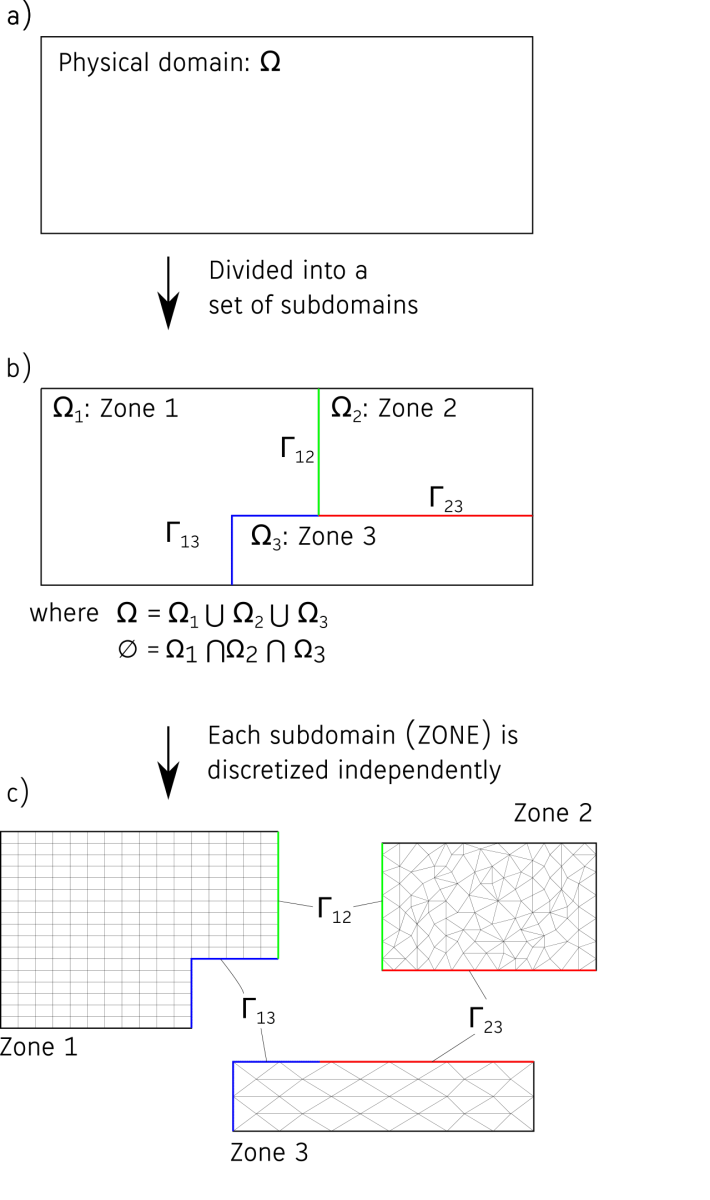
\includegraphics[width=7cm]{Figures/zones.png}
\end{center}

\subsection{Multi-zone and Multi-physics}

A multi-zone problem is a problem that consists of multiple zones. If there are additionally different physical problems solved in the individual zones (i.e. the option \verb|SOLVER| is different) then we refer to that as a multi-physics problem, otherwise we call it a single-physics problem. In that sense, every multi-physics problem is also a multi-zone problem. However, both cases differ slighty in how a problem is set up using the config files.

\subsubsection{How to set up a single-physics problem}

To enable the multi-zone mode use the option \verb|MULTIZONE = YES| (default is \verb|NO|). If all zones share all config options and are not connected, this is all you have to do. To define a common interface between zones use the option \verb|MARKER_ZONE_INTERFACE|. This option should be set to a list of markers, in which every two consecutive markers are considered as a connected pair, e.g.:

\begin{lstlisting}
MARKER_ZONE_INTERFACE= ( internal_interface, inner_interface, domain_interface, external_interface )
\end{lstlisting}


In this example \verb|internal_interface, inner_interface| and \verb|domain_interface|,\\ \verb|external_interface| are connected. The type of interface is determined automatically, depending on the type of the physical problem (set with \verb|SOLVER|).

\textbf{Note}: Currently the only single-physics problems available are Fluid-Fluid cases (that means \verb|SOLVER| must be set to \verb|EULER|/\verb|INC_EULER|, \verb|NAVIER_STOKES|/\texttt{INC\_NAVIER\_STOKES} or \verb|RANS/INC_RANS|).

\subsubsection{Sub-config files}

Even if you run a single-physics problem, there might be cases where you want to use different config options in the individual zones. For example to specify a rotation in one zone or to use a different numerical scheme. This can be accomplished using the sub-config file feature of SU2. A sub-config file is similar to the usual config file, but only contains options which are different from the main config file in the particular zone. This allows to override or to only set options in certain zones. To use this feature just provide a list of sub-config files using the \verb|CONFIG_LIST| option. The number of items in that list must match the number of zones (of course you can provide an empty file or the same file for multiple zones). The first item in that list sets options in zone 0, the second in zone 1 and so on.

As an example consider a problem with two zones coupled using a Fluid-Fluid interface. In the second zone we want to add a rotation. The two additional entries in the main config file are the following:

\begin{lstlisting}
% Enable Multizone mode
MULTIZONE= YES
%
% List of config files to specify zone options
CONFIG_LIST= (zone_0.cfg, zone_1.cfg)
%

\end{lstlisting}

In zone 0 we do not want to override any options from the main config. In particular (in contrast to zone 1) we do not want to add rotation. The file \verb|zone_0.cfg| could be very well just empty, but to make it more clear we explicitly disable any grid movement:

\begin{lstlisting}
% zone_0.cfg
% ------------------- DYNAMIC MESH DEFINITION ------------------ %
%
% Dynamic mesh simulation (NO, YES)
GRID_MOVEMENT= NONE
%

\end{lstlisting}

\verb|zone_1.cfg| contains the options to set the rotation:

\begin{lstlisting}
% zone_1.cfg
% ---------------- DYNAMIC MESH DEFINITION --------------------- %
%
% Type of dynamic mesh (NONE, ROTATING_FRAME)
GRID_MOVEMENT= RIGID_MOTION
%
% Motion mach number (non-dimensional). Used for intitializing a viscous flow
% with the Reynolds number and for computing force coeffs. with dynamic meshes.
MACH_MOTION= 0.35
%

MOTION_ORIGIN= 0.3 0.0 0.0

% Angular velocity vector (rad/s) about the motion origin. 
ROTATION_RATE = 0.0 0.0 160.0

\end{lstlisting}

\subsubsection{How to set up a multi-physics problem}

While for the single-physics problems the usage of sub-config files is optional, setting up a multi-physics problem heavily relies on this feature. A good way to start is to first create a separate config file for each individual zone. If it is possible, also try to run each zone independently (with appropriate boundary conditions) to find proper numerical settings. To couple the zones create a new config file with the option \verb|MATH_PROBLEM| set to \verb|MULTIPHYSICS|. Then specify the list of config files with \verb|CONFIG_LIST|. These two options are mandatory. To set a coupling between the zones the \verb|MARKER_ZONE_INTERFACE| option can be used (same way as for the single-physics problem). As an example consider the following main config file:

\begin{lstlisting}
% main_config.cfg
% --------------------- MULTI-PHYSICS SETUP ----------------------%
% Problem definition
PHYSICAL_PROBLEM= MULTIPHYSICS

% The list of config files
CONFIG_LIST = (configFlow.cfg, configSolid.cfg)

% The markers which should be coupled
MARKER_ZONE_INTERFACE= (PIN, PINSD)

\end{lstlisting}


The files \verb|configFlow.cfg| and \verb|configSolid.cfg| contain a full set of options to run a flow or a heat equation problem, respectively (apart from a definition of the boundary conditions for the markers \verb|PIN| and \verb|PINSD|, which will be determined automatically). However, every option not present in the sub-config files will be inherited from the main config file. If it is also not set there, then the default value will be used. This means options common in all zones, can be written to the main config file.

\subsubsection{Providing mesh information for a multi-zone problem}

For a multizone problem you have two options to provide the mesh (set with the option \verb|MULTIZONE_MESH|).

\begin{itemize}
    \item Multi-zone mesh (\verb|MULTIZONE_MESH= YES| (default)): In this case the mesh information for all zones is in one file. Note that this option currently only works with the native SU2 mesh format (\verb|MESH_FORMAT= SU2|) and the keywords \verb|NZONE=| and \verb|IZONE=| have to be present in the mesh file. Example:
    \begin{lstlisting}
% Number of zones
NZONE= 2


% Information for zone with index 1 follows
IZONE= 1
%
% Problem dimension
%
NDIME= 2
%
% Inner element connectivity
NELEM= 39092
 5  1264 1265  825    0
...

% Information for zone with index 2 follows
IZONE= 2
%
% Problem dimension
%
NDIME= 2
%
% Inner element connectivity
%
NELEM= 6365
 5   364  365  366    0
...
\end{lstlisting}
    \item  Single-zone mesh (\verb|MULTIZONE_MESH= NO|): In this case there is a separate mesh file for each zone and \verb|MESH_FILENAME| must be set in the sub-config files.
\end{itemize}

   


\newpage
\section{Execution}
Once downloaded and installed, and now that you know the basics for setting up your problems, SU2 will be ready to run simulations and design problems. Using simple command line syntax, users can execute the individual C++ programs while specifying the problem parameters in the all-purpose configuration file. For users seeking to utilize the more advanced features of the suite (such as shape optimization or adaptive mesh refinement), Python scripts that automate more complex tasks are available. Appropriate syntax and information for running the C++ modules and python scripts can be found below.

\subsection{C++ Modules}
As described in the Software Components page, there are a number of C++ modules that are the core of the SU2 suite. After compilation, each can be executed at the command line using a Unix-based terminal (or appropriate emulator, such as Cygwin). The executables for these modules can be found in the \verb|$SU2_HOME/<MODULE_NAME>/bin| directories and in the \verb|$SU2_HOME/SU2_PY| directory. The configuration file specifies the problem and solver parameters for all SU2 modules and must be included at runtime.

The syntax for running each C++ module individually in serial is:

\begin{lstlisting}
$ SU2_MODULE your_config_file.cfg
\end{lstlisting}


where \verb|SU2_MODULE| can be any of the C++ modules on the Software Components and \\ \verb|your_config_file.cfg| is the name of the configuration file that you have prepared for the problem. An example of a call to SU2\_CFD with a configuration file “default.cfg” is included below:

\begin{lstlisting}
$ ./SU2_CFD default.cfg
\end{lstlisting}


where the executable, SU2\_CFD, and the Configuration File, default.cfg, are located in the current working directory. Please see the Build from Source page for how you can set up environment variables to run the modules from any directory. Additionally, SU2 is a fully-parallel suite, and assuming that you have compiled with MPI support, each of the modules can be executed in parallel. For example, to run the CFD solver on 8 cores, you might enter:

\begin{lstlisting}
$ mpirun -n 8 SU2_CFD default.cfg
\end{lstlisting}


Note that, depending on your flavor of MPI, you may need to use a different launcher, such as mpiexec. Please see the documentation for your particular MPI implementation.

\subsection{Python Scripts}

The distribution of SU2 includes several Python scripts that coordinate the use of the C++ modules to perform more advanced analyses and simulations. A working installation of Python is highly recommended, as a number of tasks can be easily automated using provided scripts (e.g., computing a drag polar). These Python scripts can be found in the \verb|$SU2_HOME/SU2_PY|.

All of the scripts can be executed by calling python and passing the appropriate SU2 python script and options at runtime. The syntax is as follows:
\begin{lstlisting}
$ python script_name.py [options]
\end{lstlisting}


where \textit{script\_name.py} is the name of the script to be run, and \textit{[options]} is a list of options available to each script file. A brief description of the most commonly used scripts, their execution syntax, and runtime options are included below. Users are encouraged to look at the source code of the python scripts. As with many Python programs, the code is easily readable and gives the specifics of the implementation. They can also be used as templates for writing your own scripts for automating SU2 tasks.

\subsubsection{Parallel Computation Script (parallel\_computation.py)}

The parallel computation script, parallel\_computation.py, coordinates the steps necessary to run SU2\_CFD in parallel and produce solution output files. The script calls SU2\_CFD in parallel (using MPI) with the indicated number of ranks. At the conclusion of the simulation, the parallel\_computation.py script generates the solution files from the restart file written during execution by calling the SU2\_SOL module. The SU2\_SOL module can be executed at any time (in serial or parallel) to generate solution files in a specified format from a restart file and corresponding mesh.

Usage: \verb|$ python parallel_computation.py [options]|

Options:

\begin{itemize}
    \item \verb|-h, --help| show help message and exit
    \item \verb|-f FILE, --file=FILE| read config from FILE
    \item \verb|-n PARTITIONS, --partitions=PARTITIONS| number of PARTITIONS
    \item \verb|-c COMPUTE, --compute=COMPUTE| COMPUTE direct and adjoint problem
\end{itemize}
    

\subsubsection{Continuous Adjoint Gradient Calculation (continuous\_adjoint.py)}

The continuous adjoint calculation script, continuous\_adjoint.py, automates the procedure for calculating sensitivities using a continuous adjoint method. The script calls SU2\_CFD to first run a direct analysis to obtain a converged solution, then calls SU2\_CFD again to run an adjoint analysis on the converged flow solution to obtain surface sensitivities. The SU2\_DOT module is then called to project design variable perturbations onto the surface sensitivities calculated in the adjoint solution to arrive at the gradient of the objective function with respect to the specified design variables.

Usage: \verb|$ python continuous_adjoint.py [options]|

Options:

\begin{itemize}
    \item \verb|-h, --help| show help message and exit
    \item \verb|-f FILE, --file=FILE| read config from FILE
    \item \verb|-n PARTITIONS, --partitions=PARTITIONS| number of PARTITIONS
    \item \verb|-c COMPUTE, --compute=COMPUTE| COMPUTE direct and adjoint problem
    \item \verb|-s STEP, --step=STEP| DOT finite difference STEP
\end{itemize}
    

\subsubsection{Discrete Adjoint Gradient Calculation (discrete\_adjoint.py)}

Similar to the continuous adjoint script, the discrete adjoint script calls SU2\_CFD to generate a flow solution and then calls SU2\_CFD\_AD to run an adjoint computation based on the objective function specified in the config file. Finally, SU2\_DOT\_AD is called to map the surface sensitivities onto the design variables specified desig variables.

Usage: \verb|$ python discrete_adjoint.py [options]|

Options:
\begin{itemize}
    \item \verb|-h, --help| show help message and exit
    \item \verb|-f FILE, --file=FILE| read config from FILE
    \item \verb|-n PARTITIONS, --partitions=PARTITIONS| number of PARTITIONS
    \item \verb|-c COMPUTE, --compute=COMPUTE| COMPUTE direct and adjoint problem
\end{itemize}
    
\subsubsection{Finite Difference Gradient Calculation (finite\_differences.py)}

The finite difference calculation script is used to calculate the gradient of an objective function with respect to specified design variables using a finite difference method. This script calls SU2\_CFD repeatedly, perturbing the input design variables and mesh using SU2\_DEF, stores the sensitivity values, and outputs the gradient upon exit.

Usage: \verb|$ python finite_differences.py [options]|

Options:

\begin{itemize}
    \item \verb|-h, --help| show help message and exit
    \item \verb|-f FILE, --file=FILE| read config from FILE
    \item \verb|-n PARTITIONS, --partitions=PARTITIONS| number of PARTITIONS
    \item \verb|-s STEP, --step=STEP| finite difference STEP
    \item \verb|-q QUIET, --quiet=QUIET| if True, output QUIET to log files
\end{itemize}
    
    
   
    
    

\subsubsection{Shape Optimization Script (shape\_optimization.py)}

The shape optimization script coordinates and synchronizes the steps necessary to run a shape optimization problem using the design variables and objective function specified in the configuration file. The optimization is handled using SciPy’s SLSQP optimization algorithm by default. Objective functions (drag, lift, etc.) are determined by running a direct flow solution in SU2\_CFD, and gradients are obtained using the adjoint solution by default (other options can be selected). For each major iteration in the design process, the mesh is deformed using SU2\_DEF, and the sequence is repeated until a local optimum is reached.

Usage: \verb|$ python shape_optimization.py [options]|

Options:
\begin{itemize}
    \item \verb|-h, --help| show help message and exit
    \item \verb|-f FILE, --file=FILE| read config from FILE
    \item \verb|-r NAME, --name=NAME| try to restart from project file NAME
    \item \verb|-n PARTITIONS, --partitions=PARTITIONS| number of PARTITIONS
    \item \verb|-g GRADIENT, --gradient=GRADIENT| Method for computing the GRADIENT (ADJOINT, DISCRETE\_ADJOINT, FINDIFF, NONE)
    \item \verb|-q QUIET, --quiet=QUIET| True/False Quiet all SU2 output (optimizer output only)
\end{itemize}
    

\end{document}

